\section{Steepest Descent Paths}
\label{sec:sdps}

\begin{figure}[h]
  \begin{center}
    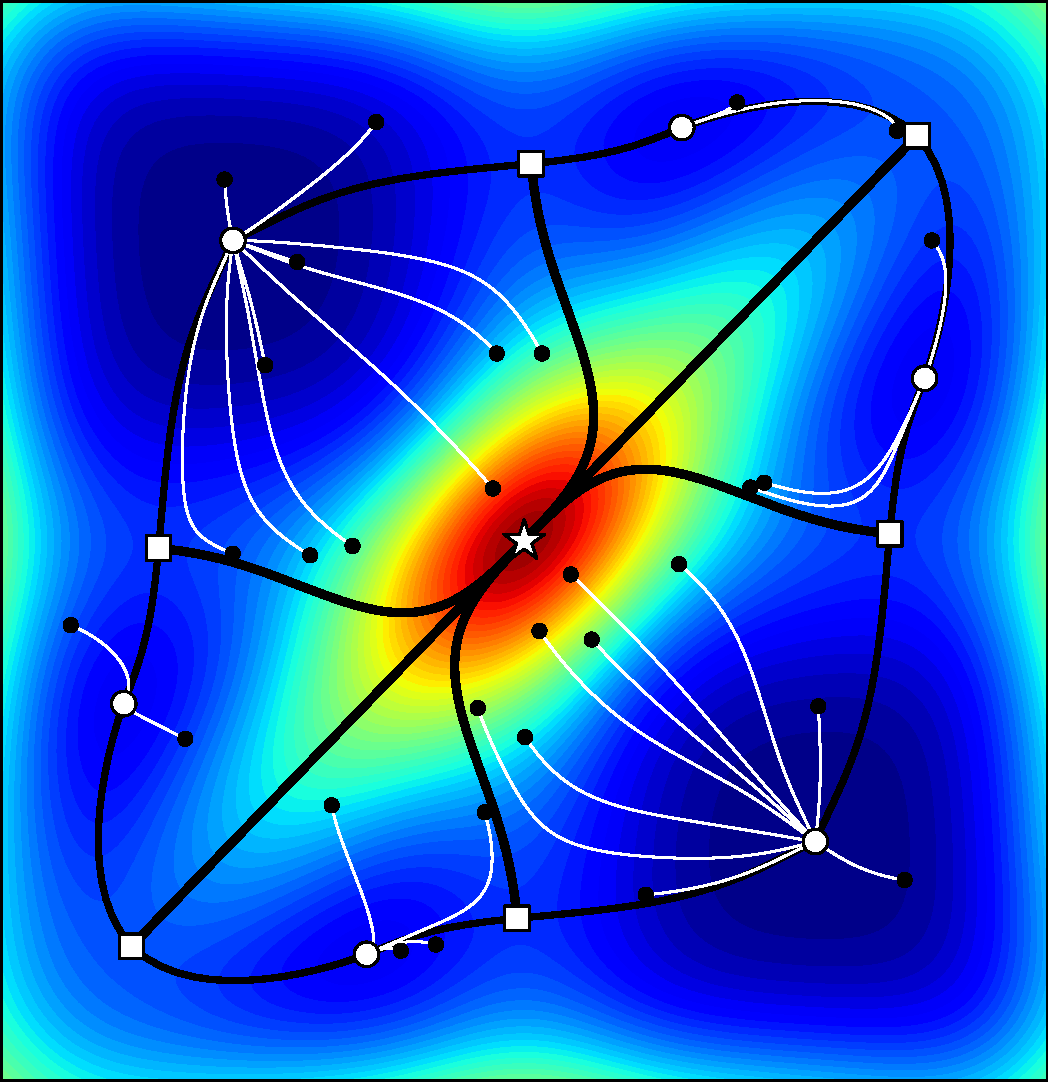
\includegraphics[width=0.6\linewidth]{paths}
    \parbox{0.85\linewidth}{
      \caption{Examples of steepest descent paths.
The white symbols represent stationary points, the circles are minima, the squares are \sap{1}s and the star is a \sap{2}.
The black circles are starting points for random SDPs (the white lines).
The black lines are specific SDPs, the dotted ones are ridges while the solid ones are MEPs.
      }
      \label{fig:paths}
    }
  \end{center}
\end{figure}

Steepest Descent Paths (SDPs) are paths on a multidimensional function, $f$, for which there is no perpendicular gradient component,
\beq{sdp-definition}
\nabla \vect{f} - (\nabla \vect{f} \cdot \uvt)\uvt = \vect{0},
\eeq
where $\uvt$ is the tangent to the path.
They can be created by following the negative gradient until it vanishes.
SDPs can begin anywhere, apart from points with a vanishing gradient, but, generally, end at minima (most common) or \sap{}s.
Two sorts of SDPs are of particular interest for the work presented in this thesis, both of which are discussed below.

%\bit
%\item Missing citation, maybe it is okay to use \cite{gradient-extremals-ruedenberg-1993}
%\eit

\subsubsection{Minimum Energy Paths}
%\label{sec:meps}

%\bit
%\item Need a good definition and/or citation.
%Check this reference:
%Transition-Path Theory and Path-Finding Algorithms for the Study of Rare Events
%(Weinan E and Eric Vanden-Eijnden)
%\eit

The Minimum Energy Path (MEP) is a collection of two specific SDPs, used in the context of theoretical reaction chemistry and represents a likely reaction path on the PES.
It leads between two minima through a \sap{1}, where each SDP begins~\cite{neb-polemic-henkelman1}, with an infinitesimal displacement along the path.

%The MEP's formal definition is generally the same as for any SDP (\fref{eq:sdp-definition}) but with the added criteria that the energy must be at a minimum perpendicular to the path~\cite{neb-polemic-henkelman1},
%\beq{mep-definition}
%\text{\expand}
%\eeq

\subsubsection{Ridges}
%\label{sec:ridges}

Similar to MEPs, ridges are collections of specific SDPs, but with their start points at a \sap{2}s and their end points in \sap{1}s.
Of course, MEPs do not exists near \sap{2}s, and the analogue ends there as the criterion for a ridge demands a negative eigenvalue in the reduced Hessian, perpendicular to the path.
